\section{Experiments}
In this section, 
% after introducing the datasets we construct from multiple business lines, 
% we discuss our experimental results under single- \& multi-domain product categorization scenarios. A brief comparison of time efficiency between $\mathsf{TaLR}$ and simple \textit{Reranking} is also included. We also discuss the generalizability of $\mathsf{TaLR}$ under zero-shot conditions (evolving taxonomy  \& new taxonomy). 
we discuss experimental results under static multi-domain settings and dynamic (taxonomy evolving \& new taxonomy) conditions. A brief comparison of time efficiency between $\mathsf{TaLR}$ and simple \textit{Reranking} is also included.

% \subsection{Dataset Analysis}

\subsection{Baselines}
\label{sec: baseline}
% \TODO{Intro: TF-IDF+LR, fastText, BERT, multi-task,...}
We implement several baseline methods based on single-domain, multi-domain, and dynamic scenarios. 
To ensure fair comparisons, we also experiment concatenating product titles with meta concept text as input for some competitive baselines.
% \subsubsection{Single-domain}
% For methods targeting single-domain categorization tasks, we train individual models for each business. 
% As a system to be deployed in production environment with limited resources, 
Note that all the strong baselines are practicable in our online production environment, and those with unbearable space or time complexity are not considered. 
% We only choose practicable baselines that meet our production environment and 
Works holding different assumptions (e.g. necessitate multi-label or not support Chinese) with us are not considered either. 
Finally, we deploy and benchmark the following common baselines: 

\textit{Flat Classifier} \textbf{TF-IDF\&LR} represents product titles with TF-IDF weighted dense vectors, and executes classification with Logistic Regression. \textbf{FastText} \cite{bojanowski2017enriching} is a common baseline adopted in online product categorization challenges. 
% We also utilize pretrained 
\textbf{BERT} classifier is used as the strong baseline in both single-domain and multi-domain (trained with multi-task learning) settings.

\textit{Hierarchical Classifier} \textbf{HMCN}~\cite{wehrmann2018hierarchical} and \textbf{HiMatch}~\cite{chen2021hierarchy} leverage hierarchical information from taxonomy to 
guide the classification process, and we use BERT as a text encoder in both approaches. 
\textbf{XR-Linear} and \textbf{XR-Transformer} are two derivatives of PECOS~\cite{yu2020pecos} framework for extreme classification, which achieve competitive performance in most open product categorization datasets.

% HiMatch implicitly models hierarchical knowledge via GCN and positive \& negative node sampling.

% \subsubsection{Multi-domain}
% We exploit \textbf{multi-task} learning paradigm as strong baseline for multi-domain categorization. 
% % A shared BERT is utilized as the text encoder with multiple output heads targeting different tasks. 
% Data batches from each task take turns to update the model weights during training, and the loss function is formulated by summing up multi-class cross-entropy losses across different tasks.
% \subsubsection{Zero-shot Setting}
% \textit{Zero-shot Classifier} Since all the above baselines cannot tackle taxonomy evolving issues
% % (evolving taxonomy  \& new taxonomy) 
% without re-training, we adopt the vanilla BERT to encode both product titles and category names and calculate their [$\mathtt{CLS}$] similarity as a naive baseline \textbf{BERT-matching}. We further utilize separate BERT classifiers trained with few-shot data (1\%) on each task respectively as a strong baseline \textbf{BERT-few-shot}. \TODO{delete and move to each sub section}
% While each component of $\mathsf{TaLR}$ could be used individually under zero-shot scenarios, the ablations of $\mathsf{TaLR}$ can also be regarded as competitive zero-shot alternatives. 

\subsection{Experimental Setup}
We mix up training data from three datasets to train the unified $\mathsf{TaLR}$. 
We use \textbf{accuracy} score as the evaluation metric to meet real-world business demands.
Accuracy mathematically equals to \textbf{Micro-F1} score in a single-label multi-class classification problem. More details can be found in Appendix~\ref{appdix:exp detail}.

\subsection{Overall Results}
\label{sec:all res}

\begin{table}[!th]
\small
\setlength{\tabcolsep}{3.5pt}
  \begin{threeparttable}[b]
  \caption{The accuracy of baselines and our $\mathsf{TaLR}$ framework with variants on static multi-domain datasets. The best results are \textbf{bolded}, and the best baseline results are starred. Overall accuracy is the weighted average w.r.t respective test set size. $\mathsf{MS}$: mapping scorer, $\mathsf{CL}$: contrastive learning. 
  % ``+concept'' means concatenation of concepts after the product title, and (-) means ablation. 
  % \xiujie{(+) ... ablation?}
  }
  \label{tb:all}
  \centering
  \begin{tabular}{l|llll}
    \toprule
    Methods & Overall & \multicolumn{1}{c}{QD} & \multicolumn{1}{l}{\;BH} & \multicolumn{1}{l}{\;FG}\\
    \midrule
    \multicolumn{5}{c}{Separate models}\\
    \midrule
    TF-IDF\&LR $ $ & 69.51 & 69.93 & 68.23 & 69.95 \\
    FastText $ $ & 74.62 & 74.01 & 71.68 & 80.82 \\
    BERT $ $ & 83.49 & 84.82 & 79.93$^*$ & 84.23\\
    BERT+$\spadesuit$  $ $ & 83.01 & 86.45 & 79.02 & 75.32\\
    % HFGN-F-classifier $ $ & - & 83.72 & 77.09 & 84.25 \\
    HMCN-F-BERT $ $ & 82.14 & 83.72 & 77.09 & 84.25 \\
    HiMatch-BERT $ $ & 84.08 & 86.12 & 77.38 & 84.19 \\
    HiMatch-BERT+$\spadesuit$$ $ & 83.75 & 87.26$^*$ & 77.26 & 78.53 \\
    XR-Linear$ $ & 76.57& 75.27 & 77.91 & 78.95 \\
    XR-Transformer$ $ & 84.58$^*$ & 79.74 & 79.23 & 84.58$^*$ \\
    XR-Transformer+$\spadesuit$$ $ & 81.45 & 85.34 & 74.59 & 78.53  \\
    \midrule
    (a): $\mathsf{TaLR}$ $ $ & 85.90 & 87.88 & 81.92 & 85.09\\
    \midrule
    \multicolumn{5}{c}{Unified model}\\
    \midrule
    % BERT Multi-task & 64.41 & 76.79 & 50.26 & 44.09 \\
    BERT Multi-task & 68.00 & 80.27 & 50.28 & 44.29 \\
    BERT Multi-task+$\spadesuit$ & 67.79 & 81.37 & 49.77 & 39.83 \\
    (b): $\mathsf{TaLR}$ & \textbf{86.23} & \textbf{88.16} & \textbf{82.48} & \textbf{85.25}\\
    \midrule
    \multicolumn{5}{c}{$\mathsf{TaLR}$ ablation test}\\
    \midrule
    % (-) rerank stage & {82.29}  & 84.19  & {77.63}  & 82.72 \\
    % (-) retrieval stage & 83.29  & 84.95  & 80.53  & {81.78} \\
    % \midrule
    % \midrule
    (c): (b) (-) $\mathsf{CL}$ & 85.26  & 86.83  & 81.75  & 85.13 \\
    (d): (b) (-) $\mathsf{MS}$ & {84.63}  & {86.59}  & {80.13}  & {84.71}  \\
    (e): (b) (-) $\mathsf{CL}$\&$\mathsf{MS}$ & 82.82 & 83.85 & 79.15 & 84.71 \\
    (f): (b) (-) $\mathsf{CL}$\&$\mathsf{MS}$ +$\spadesuit$ & 84.38 & 87.43 & 80.64 & 79.77 \\

    % (-) vector-based retrieve & 84.91  & 86.52  & 81.66  & 84.28  \\

    \bottomrule
  \end{tabular}
  \begin{tablenotes}
    % \item[1] The overall accuracy is the weighted average of results on three domains, where weights are determined by the size of their corresponding test set.
    % We list separate accuracy on each subset.
    % \item[2] Methods with $ $ notation train three separate models on the three datasets of business lines and infer using its corresponding model. Methods without $ $ only train one unified model using multi-domain data.
    % \item[3] (-) denotes the ablation of following modules in $\mathsf{TaLR}$.
    \item[$\spadesuit$] concatenate concept text after product title
    \item[(-)] ablate cretain modules
    % \item[$\mathsf{MS}$] mapping scorer module
    % \item[$\mathsf{CL}$] contrastive learning module
  \end{tablenotes}
  \end{threeparttable}
\end{table}
The overall accuracy score is shown in \tabref{tb:all}.
% , and we can make the following observations.
Since traditional single-domain approaches cannot tackle \textbf{multi-domain taxonomies}, we train \textbf{separate} models on each business respectively. 
Among methods targeting one static taxonomy, hierarchical classifiers generally perform better than flat classifiers
% mainly because it leverages 
with the aid of taxonomy structure information.
% utilizes the positive and negative relationship of nodes in taxonomy.
However, because these methods can only handle one static taxonomy, they not only suffer from efforts to maintain different models for each domain but also fail to leverage multi-domain data. 
While the multi-task BERT is able to train and infer on three domains within one model, it performs even worse than TF-IDF\&LR on BH and FG. 
One possible reason is that the multi-task approach relies heavily on the weighting of losses, and if the task-specific training data distribution varies significantly, one task might dominate the joint distribution and constrain the optimization of other tasks. 
% Straightforwardly 
Simply concatenating meta concepts to titles does not always take effect,
% for these methods on some domains, 
and this is expected since concatenated tokens implicitly contribute to the joint representation of one sentence (e.g. self-attention in transformer), which proves to be inferior to our explicit usage of statistical mapping and contrastive grouping.
% this is expected since short concept texts can not dominate the surface form of titles, and these methods does not optimize relatedness in a macroscopic view. \zelin{not clear}


For our proposed framework $\mathsf{TaLR}$, variant (a) already outperforms other baselines in separate model training paradigm, while $\mathsf{TaLR}$ (b) further achieves even higher accuracy when jointly trained on the mixed multi-domain data where the multi-task BERT fails,
verifying $\mathsf{TaLR}$'s efficacy on \textbf{multi-domain taxonomies}. 
% As is shown, the unified $\mathsf{TaLR}$ (b) is better than separate $\mathsf{TaLR}$ (a), and 
We assume that the measurement of semantic relatedness is transferable on either business domain, and their shared knowledge could be integrated via contrastive pretraining as well. 
% We assume that some products and category names from multiple domains 
% may share similar semantic meanings as well as concepts knowledge, 
Therefore, the unified training helps improving the performance on each respective domain instead of conflicting each other as BERT multi-task does. 
% This is our cross-domain \textbf{knowledge integration} assumption and is thus verified. 
% \zelin{not clear}
% \zelin{not perspicuous}
% Furthermore, when we compare $\mathsf{TaLR}$ (-) reranking (a single BERT bi-encoder) and $\mathsf{TaLR}$ (-) retrieval (a single BERT cross-encoder) with the BERT-classifier, the results is close. 
% This first elucidates that these two stages are reinforcing each other, and further corroborates that the improvement of $\mathsf{TaLR}$ from $\mathsf{TaLR}$ $ $ is contributed by the \textbf{knowledge integration} capability of the framework instead of purely addition of data.

From the ablation tests, we can observe the effectiveness of the two plug-in modules in our $\mathsf{TaLR}$ framework from row (c) and (d), and the contribution of these two modules are orthogonal. 
Removing the mapping scorer in (d) drops the overall accuracy most, 
while removing contrastive pretraining in (c) results in its inferior performance than (a) as well. 
This indicates both modules are indispensable for the enhancement of exploiting multi-domain data.
% Compared with (e)$\rightarrow$(c) and (e)$\rightarrow$(d), (e)$\rightarrow$(f) improves the least in overall accuracy, showing that our two plug-in modules are more effective than simply concatenation of concepts. 
From (e)$\rightarrow$(f), concatenating meta concepts somehow improves the overall performance, but (f) still loses to (b). This reaffirms our above assumption that our usage of meta concepts is superior to simple concatenation. 
% \zelin{no key point}
% showing that our model with concept grouping can semantically align the embeddings of product titles and category names from multiple domains. 
% Removing the concept retrieval unit impairs the overall results significantly, mainly on account of the external knowledge imported from the concept set. 
To further analyze the effects of the two plug-in modules, we conduct Case Study in Appendix~\ref{sec:appdix-case}.

\subsection{Time Consumption} 
\label{sec:time cons}
% A big concern of our framework is to limit the run-time overheads, since the large label space challenge may deteriorate in one-vs-all retrieval systems rather than classification approaches.  
To meet online deployment requirement, the inference time consumption (seconds cost for each instance) needs to be considered. We compare $\mathsf{TaLR}$ with the vanilla model (single BERT cross-encoder) on the three datasets in \figref{fig:time}.
% , and we train and test on our three standard datasets. 
% Here the single BERT cross-encoder computes the similarity score over all category classes and selects the most similar one as the prediction, while $\mathsf{TaLR}$ instead utilized bi-encoder with cached category embeddings to conduct one-vs-all retrieval and the cross-encoder BERT in \textit{Reranking} stage takes only 10 candidates. 
% \figref{fig:time} plots the relationship between the number of classes and the inference time. 
On the one hand, the inference speed of $\mathsf{TaLR}$ is much faster (4 times faster for FG and 10 times faster for BH) than vanilla model owing to the \textit{Retrieval} stage. On the other hand, the time consumption per item of $\mathsf{TaLR}$ increases almost linearly along with the number of classes, while for vanilla model the overhead grows more sharply, revealing the time efficiency of $\mathsf{TaLR}$ when the class number scales up. 
% As for the accuracy score, $\mathsf{TaLR}$ fluctuates in the same pace with BERT cross-encoder but consistently outperforms it, and the reason of fluctuation is explained before.
% $\mathsf{TaLR}$ also consistently outperforms single BERT cross-encoder in accuracy due to the selection of better candidates in \textit{Retrieval} stage. 

\begin{figure}[thbp] \centering
    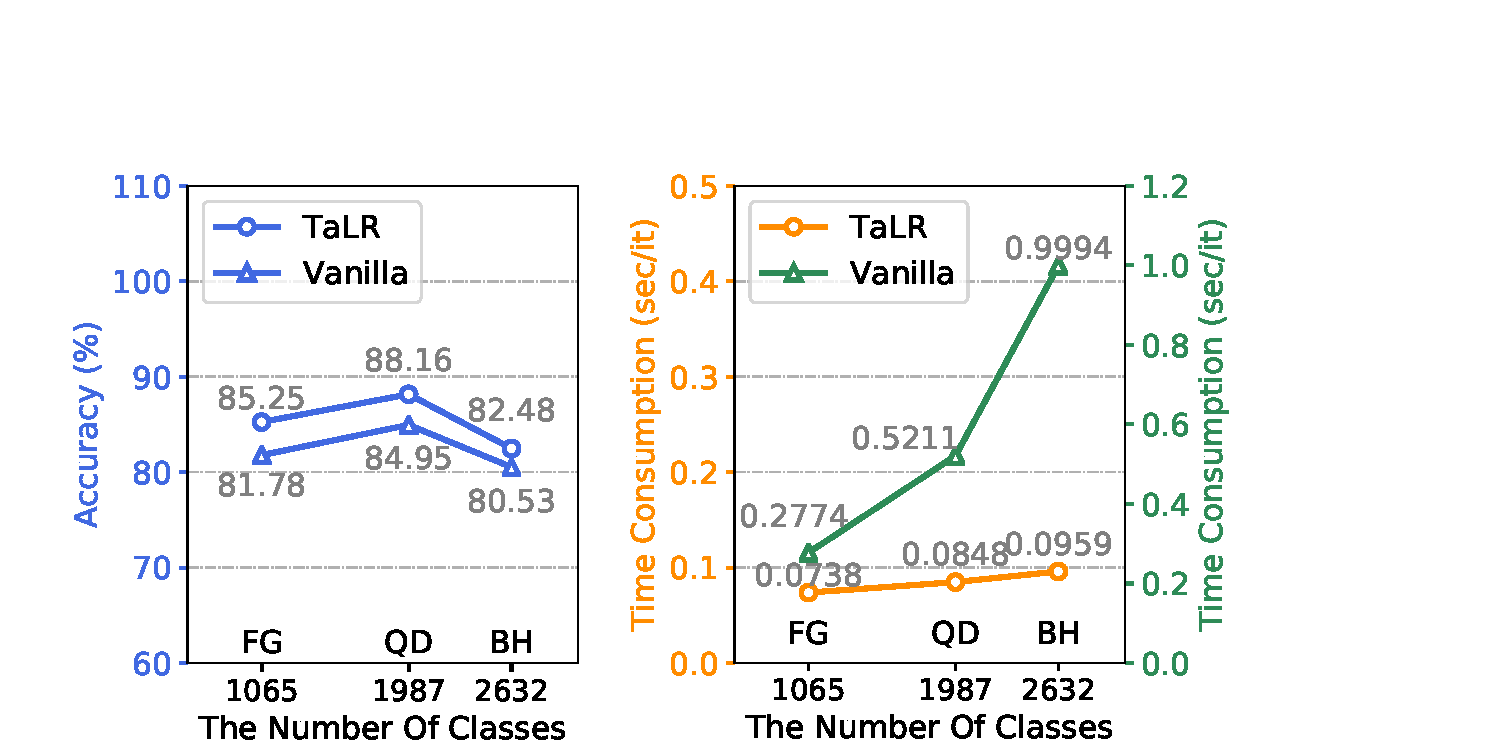
\includegraphics[width=0.4\textwidth]{time.pdf}
    \caption{Accuracy results and inference time consumption when the number of classes grows.} 
    \label{fig:time}
\end{figure}

\subsection{Dynamic Test Set Experiment}
\label{sec:evolve res}
In order to evaluate the ability of our framework on \textbf{taxonomy evolving} challenge, 
we use $\mathsf{TaLR}$ trained on the original multi-domain datasets to directly infer on two dynamic test sets. The vanilla BERT without any finetuning is a naive baseline \textbf{BERT-matching}. The BERT fine-tuned with few-shot new data (1\%) is a strong baseline \textbf{BERT-few-shot}.
% we directly infer product titles with $\mathsf{TaLR}$ trained on multi-domain datasets on the evolved taxonomies.
% we conduct experiments to directly infer evolved new category of the product with $\mathsf{TaLR}$. 
Here ``before'' denotes the subset from the original test set and ``after'' denotes the subset with the same product titles but evolved categories.
From the listed accuracy ``before'' and ``after'' taxonomy evolving in \tabref{tb:evolve}, we can conclude that $\mathsf{TaLR}$ sustains satisfactory accuracy compared with its strong counterpart trained with 1\% extra data.
% the encoded [$\mathtt{CLS}$] token similarity from %%% explained before
% BERT-matching is the vanilla similarity matching baseline and BERT-few-shot is the separate few-shot classifiers we mentioned in \secref{sec: baseline}. Note that BERT-few-shot is trained on full data before evolving.

\begin{table}[th]
\small
\setlength{\tabcolsep}{1.8pt}
  \begin{threeparttable}[b]
  \caption{The accuracy on two dynamic test sets. $\Delta$ is the change
  of accuracy after evolving. The best ``after'' scores and least drop $\Delta$ are bolded.}
  \label{tb:evolve}
  \centering
  \begin{tabular}{l|ccc|ccc}
    \toprule
    \multirow{2}{*}{Methods} & \multicolumn{3}{c|}{QD$-divide$} & \multicolumn{3}{c}{QD$-integrate$}\\
    \cline{2-7}
    & Before & After & $\Delta$ & Before & After & $\Delta$ \\
    \midrule
    BERT-matching & 6.66 & 11.95 & \textbf{+5.29} & 13.39 & 2.23 & -11.16\\
    BERT-few-shot & 90.51 & 43.54 & -46.96 & 86.79 & 50.16 & -36.53\\
    \midrule
    $\mathsf{TaLR}$ & 90.11 & \textbf{69.71} & -20.40 & 85.20 & \textbf{81.48} & \textbf{-3.72}\\
    % (-) contrastive  & 89.10 & \textbf{79.21} & -9.89 & 84.11 & 80.02 & -4.09\\
    % (-) rerank stage & 89.70 & 73.94 & -15.76 & 86.36 & 81.47 & -4.89\\
    % (-) rule-based unit & 89.51 & 64.25 & -25.26 & 84.61 & 81.19 & \textbf{-3.42}\\
    \bottomrule
  \end{tabular}
%   \begin{tablenotes}
%     \item[1] 
%   \end{tablenotes}
  \end{threeparttable}
\end{table}
% {too long, rewrite}
% On the one hand, our $\mathsf{TaLR}$ even outperforms BERT-few-shot without additional training on evolved taxonomies, which indicates its robustness in handling dynamic issues.
% On the other hand, we can observe an opposite trend of BERT-matching and $\mathsf{TaLR}$ through $\Delta$ when two different evolving challenges are encountered. In the node $integrate$ scenarios, $\mathsf{TaLR}$ exhibits robustness with a slight drop of accuracy. 
% When progressively ablating contrastive learning and the whole \textit{Reranking} stage, the accuracy of $\mathsf{TaLR}$ consistently decreases, which indicates their contributions to the node \textit{integrate} variants in evolving taxonomy.
% % \textbf{Taxonomy integration}.
% % On the other hand, BERT-matching suffers from a drastic drop in accuracy, which may attribute to 
% However in the node $divide$ scenario, wherever contrastive learning is incorporated, there is a substantial drop in $\Delta$. Completely excluding the contrastive learning while keeping all other components gives the best accuracy. 
% The reason behind it is that contrastive learning tends to make the representations of products from the same category tied closer, while the division of nodes breaks this relation. 


\subsection{Extrapolating Results on New Taxonomy}
\label{sec:new tax}

% For multi-domain business lines, 
Consider an extreme \textbf{taxonomy evolving} condition when a new business line emerges, a robust model is supposed to categorize incoming products based on the brand-new taxonomy. 
% Hence it poses challenge for $\mathsf{TaLR}$ to zero-shot transfer to new domains so as to improve user experience in this cold-start scenario.

\begin{table}[th]
%   \begin{threeparttable}[b]
  \small
  \caption{The accuracy of $\mathsf{TaLR}$ on the new taxonomy. }
  \label{tb:zeroshot}
  \centering
  \begin{tabular}{l|ccc}
    \toprule
    Methods & QD & BH & FG \\
    \midrule
    BERT-matching & 9.00 & 11.23 & 4.03 \\
    BERT-few-shot & 43.29 & 35.19 & 29.80 \\
    % BERT-product & 52.00 & 48.81 & 51.32 \\
    \midrule
    $\mathsf{TaLR}$ & \textbf{60.57} & \textbf{65.45} & \textbf{62.69}\\
    % $\mathsf{TaLR}$-few(?) &  &  & \\
    % $\mathsf{TaLR}$-finetune(?) & 84.32 & 76.40 & 83.59\\
    % \midrule
    (-) contrastive & 56.71 & 64.99 & 60.79\\
    % (-) Rerank stage & 53.79 & 59.56 & 57.68 \\
    (-) mapping scorer & 56.25 & 64.65 & 59.29\\
    \bottomrule
  \end{tabular}
%   \begin{tablenotes}
%     \item[1] 
%   \end{tablenotes}
%   \end{threeparttable}
\end{table}

We deploy our experiments in a zero-shot manner, where we take turns to train $\mathsf{TaLR}$ on either two business data and test its performance on the remaining business. $\mathsf{TaLR}$ still outperforms BERT-few-shot. 
% We compare $TaLR$ with BERT-matching model and bi-encoder BERT in zero-shot, and $TaLR$-zero sustains better accuracy, 
% This indicates that $\mathsf{TaLR}$'s ability capturing semantic relatedness between product titles and category names on original domains could be seamlessly transferred to new domains with new taxonomies.
This shows $\mathsf{TaLR}$'s preeminent transferability with the reformulation of textual semantic matching, which helps improving user experience in this cold-start scenario.
% It mainly contributes to the learning in the other two domains, 
% which enhances the semantic relatedness understanding in the third dataset with brand new taxonomy.
Each component in the ablation test verifies its effectiveness as well. 

% More details about ablation setting is in \secref{sec:exp detail}.



% \subsection{Different Retrieval Strategies}
% \label{sec:retri stra}
% In \textit{Retrieval} stage, it is encouraged to exploit the potential candidates as accurately as possible, otherwise the latter \textit{Reranking} stage would never make right predictions if the true label is not covered by the retrieved candidates. Hence we use HR@$k$ to measure the retrieval performance.

% Firstly, we compare several alternatives of the loss function in vector-based retrieval model. In \figref{fig:vector-retri}, as $k$ goes on, the HR score increases, and the model trained with Cosent loss is consistently better than others, while the model trained with SBERT loss performs unstably, sometimes worse than Cosine loss. 
% One explanation is that comparing with Cosine loss and SBERT loss, the Cosent loss focuses on the positive-versus-negative pairwise optimization, which means the model only cares for the relative order of the prediction results instead of the specific value. And this setting brings consistent recall of candidates.
% \begin{table}[th]
%   \caption{The retrieval results of the vector-based unit over different loss function. The best results are bolded.}
%   \label{tb:vector-retrieval}
%   \centering
%   \begin{tabular}{c|c|ccc}
%     \toprule
%     Loss & Dataset & HR@1 & HR@5 & HR@10 \\
%     \midrule
%     \multirow{3}{*}{Cosine} & QD & 74.80 & 82.28 & 84.46\\
%     & BH & 72.75 & 81.77& 84.04\\
%     & FG & 65.59 & 80.40 & 83.23\\
%     \midrule
%     \multirow{3}{*}{SBERT} & QD & 82.25 & 88.96 & 90.92\\
%     & BH & 76.95 & 86.76 & 89.41\\
%     & FG & 80.67 & 87.27 & 88.86\\
%     \midrule
%     \multirow{3}{*}{Cosent} & QD & 84.19 & 88.97 & 90.30\\
%     & BH & 77.64 & 85.27 & 87.18\\
%     & FG & 82.72 & 86.66 & 87.48\\
%     \bottomrule
%   \end{tabular}
% \end{table}

% \begin{figure}
%   \begin{subfigure}[b]{0.49\columnwidth}
%   \centering
%   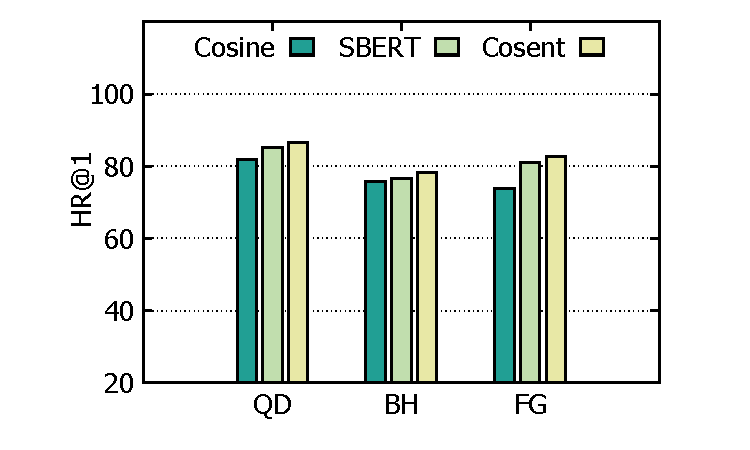
\includegraphics[width=\columnwidth]{hr_1.pdf}
%   \caption{HR@1}
%   \end{subfigure}
% %   \hfill
% %   \begin{subfigure}[b]{0.49\columnwidth}
% %   \centering
% %   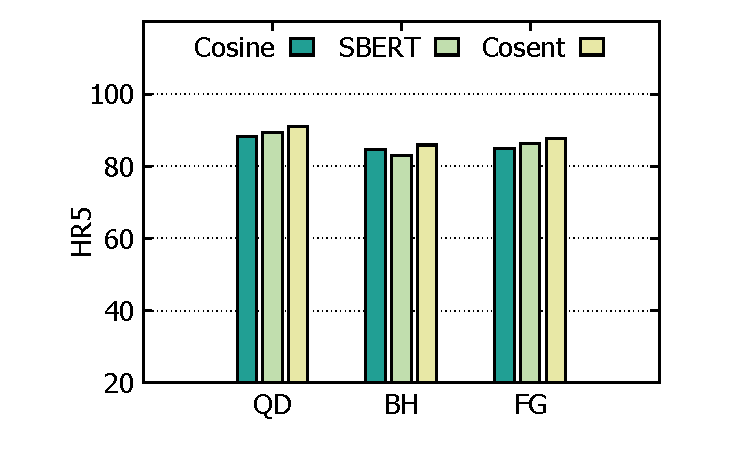
\includegraphics[width=\columnwidth]{hr_5.pdf}
% %   \caption{HR@5}
% %   \end{subfigure}
%   \hfill
%   \begin{subfigure}[b]{0.49\columnwidth}
%   \centering
%   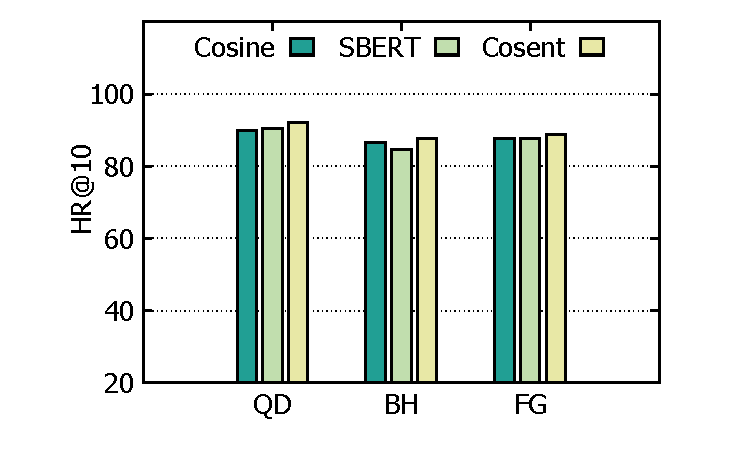
\includegraphics[width=\columnwidth]{hr_10.pdf}
%   \caption{HR@10}
%   \end{subfigure}
%   \caption{The retrieval results of the vector-based unit over different loss functions.}
%   \label{fig:vector-retri}
% \end{figure}

\cut{
To generate better candidates, we adopt several heuristic algorithms for two-way candidates fusion.
% the vector-based unit and rule-based unit. 
\tabref{tb:fusion} depicts the retrieval results over different fusion strategies. The size of merged candidate sets is not stuck to $10$ for some of the strategies, so we list the average number.
Generally, the \textbf{Rule-First} algorithm achieves better scores, and \textbf{De-Dupli} algorithm is competitive with it. We use \textbf{Rule-First} in our framework due to its fixed candidate size which is more convenient to process.
Although the pure vector-based unit performs less effectively than the rule-based counterpart, they could complement each other after fusing together with the help of an ensembled understanding of textual semantics and training set distribution.
% the ensemble of vector-based unit and rule-based unit strengthens the performance of rule-based unit, revealing that vector-based unit can better understand the instance semantically that rule-base unit can not. 
More discussions are in Case Study.

\begin{table}[th]
\setlength{\tabcolsep}{2pt}
  \caption{The retrieval results of candidates for different fusion strategies. The best results are bolded.}
  \label{tb:fusion}
  \centering
  \begin{tabular}{c|cc|cc|cc}
    \toprule
    \multirow{2}{*}{Strategy}  & \multicolumn{2}{c|}{QD} & \multicolumn{2}{c|}{BH} & \multicolumn{2}{c}{FG} \\
    \cline{2-7} 
      & Recall & Size & Recall & Size & Recall & Size \\
    \midrule
    Rule-based & 95.33 & 8.6 & 96.77 & 8.8 & 97.32 & 9.0 \\
    Vec-based & 90.30 & 10 & 87.18 & 10 & 87.48 & 10 \\
    \midrule
    De-Dupli & 96.08 & 10.5 & \textbf{97.54} & 10.4 & 97.77 & 10.7 \\
    Norm\&Rank & 93.74 & 10 & 92.42 & 10 & 92.77 & 10 \\
    Rule-First & \textbf{96.12} & 10 & 97.48 & 10 & \textbf{98.01} & 10 \\
    \bottomrule
  \end{tabular}
\end{table}
}
% \section{Case Study}
% For product ``\textit{red dancing shoes (size 35)}'', which should be categorized to \verb|Sports/Outdoors| $\rightarrow$ \verb|Yoga/Dancing| $\rightarrow$ \verb|Dancing Shoes|, the vector-based unit retrieves the correct class as top-$1$ answer, but the rule-base unit retrieves \verb|Clothes/Shoes| $\rightarrow$ \verb|Woman Shoes| $\rightarrow$ \verb|Woman Slippers| as top-$1$. This time the distribution knowledge guides the rule-based model towards a wrong direction, while the vector-based model succeeds relying on the semantic similarity.

% For product ``\textit{CHEERS$^\circledR$ 12 years}'', the vector-based model categorizes it to \verb|Books| $\rightarrow$ \verb|Economics/Management| $\rightarrow$ \verb|Marketing|, whereas the rule-based unit correctly retrieves \verb|Alcoholic Drinks| $\rightarrow$ \verb|Imported Liquors| $\rightarrow$ \verb|Whisky|. This shows that ``12 years'' misleads the vector-based model to the semantic meaning of economics, and rule-based unit successfully leverages its distribution knowledge in training set.

% For product ``\textit{towel gourd\&soy bean (towel gourd 1 pcs, soy bean 150g)}'', both rule-based unit and vector-based unit predict
% \verb|Vegetable| $\rightarrow$ \verb|Soy Product| $\rightarrow$ \verb|Soy Bean| wrongly as top-$1$, whereas $\mathsf{TaLR}$ classifies it to correct \verb|Vegetable| $\rightarrow$ \verb|Mixed Product| $\rightarrow$ \texttt{Vegetables mixture}, and clearly, the contribution is from the following \textit{Reranking} stage.
% \begin{table*}[t]
%   \caption{The retrieval results of candidates for different fusion strategies. The best results are bolded.}
%   \label{tb:fusion}
%   \centering
%   \begin{tabular}{c|c}
%     \toprule
%     Product title & \textit{red dancing shoes (size 35)} \\
%     \midrule
%     Ground truth & \verb|Sports/Outdoors| $\rightarrow$ \verb|Yoga/Dancing| $\rightarrow$ \verb|Dancing Shoes| \\
%     Vector-based top-$1$ & \verb|Sports/Outdoors| $\rightarrow$ \verb|Yoga/Dancing| $\rightarrow$ \verb|Dancing Shoes| \\
%     Rule-based top-$1$ & \verb|Clothes/Shoes| $\rightarrow$ \verb|Woman Shoes| $\rightarrow$ \verb|Woman Slippers| \\
%     \midrule
%     Product title & \textit{CHEERS$^\circledR$ 12 years} \\
%     \midrule
%     Ground truth & \verb|Alcoholic Drinks| $\rightarrow$ \verb|Imported Liquors| $\rightarrow$ \verb|Whisky| \\
%     Vector-based top-$1$ & \verb|Books| $\rightarrow$ \verb|Economics/Management| $\rightarrow$ \verb|Marketing| \\
%     Rule-based top-$1$ & \verb|Alcoholic Drinks| $\rightarrow$ \verb|Imported Liquors| $\rightarrow$ \verb|Whisky| \\
%     \midrule
%     Product title & \textit{towel gourd \& soy bean (towel gourd 1 pcs, soy bean ~150g)} \\
%     \midrule
%     Ground truth & \verb|Vegetable&/ Product| $\rightarrow$ \verb|Mixed Product| $\rightarrow$ \verb|Vegetables mixture| \\
%     Vector-based top-$1$ & \verb|Vegetable/&Soy Product| $\rightarrow$ \verb|Soy Product| $\rightarrow$ \verb|Soy Bean| \\
%     Rule-based top-$1$ & \verb|Vegetable/Soy Product| $\rightarrow$ \verb|Soy Product| $\rightarrow$ \verb|Soy Bean| \\
%     \bottomrule
%   \end{tabular}
% \end{table*}



\subsection{Online Experiment}
% We conduct online experiments on one downstream task where the category of a product is needed, 
% % of semantic vector space, 
% that is the main page recommendation (multi-domain). 
% % After deploying our contrastive pretrained model to compute the hidden vector representations of related products and utilizing this in sophisticated 
% When $\mathsf{TaLR}$ is incorporated in the
% recommendation system, customer purchase click rate increases significantly over 5\%.
We conduct online experiments on one downstream task where $\mathsf{TaLR}$'s domain-independent category recognition ability helps transfer user preferences from other domains and contributes to a more accurate recommendation. When $\mathsf{TaLR}$ is incorporated in the recommendation system, customer seasonal purchase revenue increases significantly over 5\%.